\chapter{Relatività Speciale}

\section{Un problema luminoso}

La luce non si comporta secondo la relatività galileiana: ecco, questa è la cruda verità. Macchine, proiettili, missili, ogni cosa sembra rispettare le indicazioni di Galileo tranne la luce\footnote{In realtà scopriremo come tutte le cose \textbf{non} rispettino la relatività galileiana ma ci vadano solo vicino quando le velocità siano piccole rispetto alla luce. In altri termini la relatività galileiana approssima il vero comportamento dei corpi in movimento: minore la velocità e minore sarà l'approssimazione.}.

Per evitare fraintendimenti iniziamo dai dati di fatto tornando sul nostro treno: se  sparassimo un raggio di luce invece che lanciare la nostra cara pallina ci ritroveremo subito in un bel guaio perché la velocità della luce sarebbe la stessa anche per la signora sulla pensilina. 

Sì, è assurdo e sì, il treno si muove eppure le cose stanno così.

Ripeto, la velocità della luce misurata sul treno in movimento\footnote{In movimento rispetto alla donna ferma alla banchina.} coinciderebbe con quella misurata dalla signora sulla pensilina: da qui muove l’opera di Einstein cercando di spiegare questa anomalia. 

\begin{figure}[h!]
 \centering
 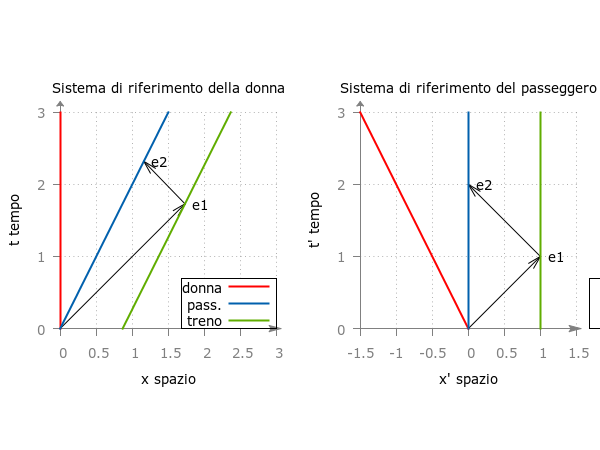
\includegraphics[scale=0.7]{figure/fig8}
 \caption{relatività galileiana}
\end{figure}



Studieremo la cosa da diversi punti di vista, prima però rifacciamo l’esperimento utilizzando la luce invece che una pallina per avere dei dati sotto mano: useremo sempre gli stessi simboli per non confonderci, modificandone però il significato. Ad esempio il treno sarà sempre lungo $c$ però questa volta $c$ indica la distanza percorsa dalla luce in un secondo, qualcosa come $299.792.458$ metri, quasi $300$ mila chilometri al secondo! Dobbiamo utilizzare grandezze così enormi altrimenti non riusciamo ad inquadrare facilmente il punto su cui ragioniamo. La velocità del treno sarà ancora $v=c/2$, $150.000$ metri ogni secondo: con una velocità del genere possiamo confidare di non avere più treni in ritardo, forse;-)

Facciamo i conti: per il passeggero tutto rimane invariato, il raggio di luce impiega $1$ secondo a percorrere la distanza $c$, quindi tutto come prima: in $2$ secondi torna indietro. Evviva!

Per la signora sulla pensilina però la luce emessa dal treno si muove a $c$, non più a $c+v$ come dovrebbe accadere secondo Galileo. Per  inseguire la testa del treno che si allontana a velocità $v$ il raggio di luce ci mette più di un secondo. Ripeto: se la testa del treno stesse ferma il raggio di luce ci metterebbe $1$ secondo a raggiungerla, ma si muove, si allontana quindi ci mette qualcosa di più di un secondo, precisamente: 1,73 secondi.\footnote{Nell'appendice, per chi ha voglia, si possono seguire i calcoli e scoprire che il tempo trascorso è $c^2/\beta$ dove $\beta= c-v$, data la velocità del treno è una costante che ritroveremo in diversi punti del nostro ragionamento: tanto vale fare la conoscenza e notare come $\beta<1$ dal momento che ogni oggetto si muove ad una velocità $v$ minore di quella della luce $c$.}. Anche a fare il giro completo ci impiega più di due secondi, 2,32 per l'esattezza. Nel grafico questo disallineamento degli eventi $e1$ e$e2$ è particolarmente evidente: nel modello galileiano differivano solo per lo spazio adesso invece anche i tempi non coincidono.

Possiamo già fermarci e riflettere sul fatto che lo stesso accadimento, lo stesso evento, avvenga dopo un secondo per il passeggero ma più tardi per la signora sulla pensilina: lo stesso \textbf{identico} evento non è più simultaneo per i due osservatori. 

Il trionfo dell'assurdità: benvenuti nell'universo relativistico in cui, d'altronde, vivete dal giorno in cui siete nati!

\section{Relatività del tempo, 1}

Magari abbiamo sbagliato i calcoli, può essere. Così hanno pensato i fisici di fronte ai risultati di molti esperimenti anche precedenti alla formulazione di Einstein: non è possibile che lo stesso evento avvenga in tempi diversi. L'esperienza di tutti i giorni ci dice esattamente il contrario... proprio come l'esperienza quotidiana dava ragione ad Aristotele circa lo stato naturale dei corpi.

Però Aristotele aveva torto, come sappiamo, e Galileo ragione, cosa che ci porta ad accettare la realtà anche se apparentemente strana e priva di senso. Quindi torniamo ai fatti: l'evento definibile come “il raggio di luce tocca la testa del treno” che chiamiamo $e1$ si comporta in modo strano, avviene prima per il passeggero e poi per la signora. Il problema non è $e1$, ma la velocità della luce che rimane costante per la donna, come abbiamo visto. Da questa inspiegabile invarianza ne deriva che il tempo trascorso per la donna, indichiamolo con $\Delta t$ è più lungo del tempo trascorso per il passeggero $\Delta t'$, per lui il tempo scorre più lento, a quanto pare. Se la signora potesse sbirciare nel treno in movimento vedrebbe ogni cosa al suo interno muoversi al rallentatore, compreso il battito cardiaco del passeggero.

Lo so, non ci credete: nessuno d'altronde credeva ad Einstein. In molti, per molti hanno hanno tentato di confutare in tutti i modi sperimentabili la sua teoria. Una volta hanno sincronizzato due orologi atomici, i più precisi di cui disponiamo, e piazzato uno dei due su un aeroplano che ha voluto in giro per il mondo. Il punto qui è che si muoveva rispetto al gemello fermo anche se a velocità piccole rispetto a quelle della luce. Eppure, tornato alla base, i due orologi non erano più sincronizzati: il viaggiatore era in ritardo rispetto a quello fermo\footnote{L'aereo girava intorno alla terra quindi non si muoveva in moto rettilineo uniforme: i discorsi sulla relatività che faremo più avanti quindi valgono solo per metà ;-)}.

Quindi il tempo è un concetto relativo come la velocità galileiana, come l'alto ed il basso, come il vicino o il lontano. Rifletteteci sopra un po' prima di procedere... intanto vi intrattengo con un altro esempio preso dalla realtà: parliamo di GPS, quel sistema che consente al vostro navigatore o cellulare di dirvi dove vi trovate sulla terra con un'ottima approssimazione. Forse non sapete che si basa su una rete di 24 satelliti che gravitano attorno al mondo in modo tale che almeno quattro siano sempre visibili da ogni luogo terrestre. Sono come dei fari per i marinai: ricevendo il loro segnale, sapendo quando lo hanno inviato e quanto tempo ci abbiamo messo a riceverlo riusciamo a scoprire quando siamo distanti da loro. 

Il punto è che l'accuratezza nel misurare il tempo è fondamentale per il funzionamento di tutto il sistema ed è qui che entra in gioco Einstein: in questi satelliti ci sono degli orologi che, udite udite, perdono tempo rispetto a quelli a terra secondo le predizioni della teoria che stiamo studiando\footnote {E anche per gli effetti di dilatazione del tempo dovuti alla gravità che non studieremo ma sono spiegati sempre da Einstein nella Teoria della Relatività Generale.}. Questo errore è compensato in modo da sincronizzare gli orologi e grazie ad Einstein abbiamo i navigatori satellitari! 

Meditate.

\section{Relatività di Einstein}

Parlando di relatività galileiana abbiamo imparato ad utilizzare un metodo grafico per ricavare le coordinate del passeggero $t',x'$ restando nella rappresentazione della signora. Possiamo fare lo stesso anche occupandoci della relatività di Einstein.


\begin{figure}[h!]
 \centering
 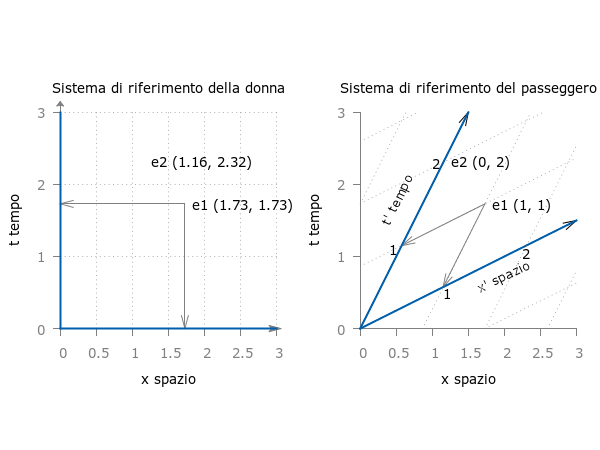
\includegraphics[scale=0.7]{figure/fig10}
 \caption{relatività galileiana}
\end{figure}

I due eventi si trovano in entrambi i grafici nella stessa posizione, il procedimento per ottenere le coordinate rimane il solito ovvero si seguono le frecce fino ai nuovi assi: l'unica incredibile differenza è che qui, dato un evento, passando da un sistema all'altro non si modifica solo la posizione nello spazio ma anche il tempo. Vi invito a notare l'asse $x'$ che è l'insieme di tutti gli eventi nell'universo per cui, per il passeggero, il tempo vale $t'=0$. In altre parole sono tutti gli eventi contemporanei al momento della sincronizzazione per il passeggero. Vi prego di notare come non sia più una curva piatta ma abbia un'inclinazione pari alla velocità $v$ del treno.

Sopra questo asse, e parallele a questo, abbiamo invece altre linee che raggruppano eventi contemporanei: avremo la linea di tutti gli eventi quando il tempo è pari a $1$ secondo, pari a $2$ e così via, una sopra l'altra (sono le linee tratteggiate parallele a $x'$.

Questa differenza di prospettiva per cui per la signora gli eventi contemporanei sono indicati da linee piatte e per il passeggero invece sono inclinate porta al risultato che, gli stessi eventi, hanno tempi diversi per i nostri due personaggi.

Provate ad allenarvi trovando le coordinate per $e1$ e $e2$ per i diversi sistemi di riferimento utilizzando un unico grafico.


\section{Spazio-tempo}

Nel nostro esperimento relativistico gli orologi sul treno sono sincronizzati con quello del viaggiatore utilizzando un raggio di luce, come abbiamo spiegato nella sezione precedente. Lo stesso è stato fatto per gli orologi sulla banchina: sono tutti coincidenti con quello della donna.

\begin{figure}[h!]
 \centering
 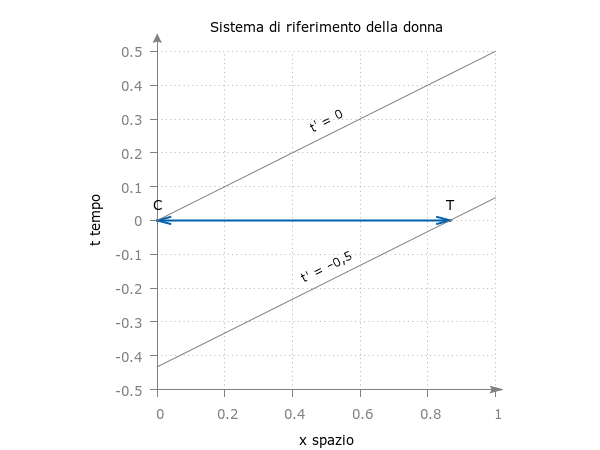
\includegraphics[scale=0.7]{figure/fig9}
 \caption{relatività galileiana}
\end{figure}

Nella figura qui sopra il treno, al momento della sincronizzazione degli orologi, è rappresentato con la linea blu orizzontale \footnote{I più attenti noteranno che il treno sia un po' più corto di $c$: non è uno sbaglio ma ne parleremo più avanti.} che va dall'evento $C$, coda del treno incrocia banchina, all'evento $T$, testa del treno incrocia fine banchina. Ricordo che il passeggero si trova in coda al treno.

Le due linea parallele sopra è sotto il treno nel nostro grafico le abbiamo conosciute nel paragrafo precedente e mostrano rispettivamente gli eventi che per il passeggero sono contemporanei a $t'=0$ e $t'=-0,5$. Tra queste due ci sono infinite linee parallele per i secondi tra $-0.5$ e $0$.

Il dato che emerge è che dopo la sincronizzazione avvenuta in $C$ per la donna, nello stesso istante, anche l'orologio in $T$ segna $0$. Normale, direte voi: già peccato però che potendo vedere dentro il treno in $T$ vedremo l'orologio del passeggero segnare un tempo precedente a zero,  $-0.5$!

La lezione è che con la caduta del tempo assoluto non esiste più uno spazio ed un tempo unico per tutti ma una cosa che è l'unione dei due, chiamata spazio-tempo costituita in ogni punto nelle spazio E nel tempo. Si tratta dei nostri eventi, come $C$ e $T$.

Il tempo e lo spazio sono mescolati in quantità diverse per osservatori diversi ma lo spazio-tempo è invariante per tutti.

Riflettete su questa importante lezione: il punto è che eventi simultanei per un osservatore non lo sono per un altro (le linee parallele piatte contro quelle inclinate). Ne deriva ad esempio che spostandosi lungo il treno nello stesso istante $t=0$ (per la signora) vedremo orologi sul treno avere orari diversi, via via minori, perché per il passeggero quegli eventi non sono contemporanei a $C$.


\section{Relatività del tempo, 2}

Il moto, lo abbiamo visto, è un concetto relativo sotto diversi punti di vista. Non solo dipende dagli osservatori, ma è anche del tutto impossibile capire per uno di loro se sia in moto (rettilineo uniforme) oppure fermo. Nessuna evidenza fisica, nessun esperimento può risolvere il problema: è l'essenza stessa del concetto relatività.

Anche la relatività del tempo per Einstein si conforma alla stessa regola: abbiamo detto che il tempo è rallentato per l'oggetto in movimento. Questo non significa solo che la signora, potendo vedere nel treno, vedrebbe tutto rallentato ma significa anche che se il passeggero guardasse la donna e la pensilina vedrebbe tutto rallentato allo stesso modo.

Se così non fosse due osservatori potrebbero confrontarsi, quello il cui tempo non rallenti sarebbe fermo ed il concetto di moto diventerebbe assoluto. Cosa che non è.

Problema: nell'esempio citato precedentemente dei due orologi atomici solo uno era rimasto indietro, contravvenendo al discorso che stiamo facendo. O forse no? No, infatti: la relatività del moto e del tempo è simmetrica solo nel caso in cui i sistemi di riferimento siano inerziali, cioè si muovano in moto rettilineo uniforme l'uno rispetto agli altri, ovvero non abbiano accelerazioni. Questo non è il caso di un aereo che curvi attorno al mondo, decolli, atterri acceleri, deceleri. 

Appena si abbandona il sistema inerziale tutta la simmetria della relatività si interrompe portando a situazioni bizzarre come il famoso paraddose dei gemelli. Lo conoscete? Uno dei due gemelli parte per un viaggio interplanetario fino ad una stella lontana, gira attorno a questo traguardo e poi torna indietro. Sbarcato si scoprirà più giovane del gemello rimasto a terra perché per lui il tempo è passato più lentamente. La mancanza di simmetria deriva dal fatto che per tornare indietro la nave ha dovuto rinunciare al moto rettilineo uniforme, ha cambiato direzione, ha subito delle accelerazioni e la simmetria della dilatazione del tempo si è spezzata.


\section{Relatività del tempo, 3}

I più attenti tra voi avranno notato un'incongruenza logica nel paragrafo precedente: se per la donna il tempo del passeggero è rallentato... come fa per questi ad essere il tempo della donna rallentato? È impossibile, illogico sbagliato. Nel nostro esperimento l'evento $e2$ accade dopo $2.32$ secondi per la signora e, abbiamo visto, dopo soli $2$ secondi per il passeggero. Quindi quando per il passeggero passano $2$ secondi per la donna passano $2.32$? Cade la simmetria della relatività?

No, stiamo solo sbagliando a confrontare gli orologi ignorando completamente il concetto di spazio-tempo illustrato qualche paragrafo più indietro. Iniziamo spiegando quale dovrebbe essere la sequenza logica per confrontare gli orologi:

\begin{enumerate}
 \item quando il mio orologio segna un certo tempo...
 \item dove si trova l'orologio con cui mi sono sincronizzato e...
 \item che ora segna? 
\end{enumerate}

\begin{figure}[h!]
 \centering
 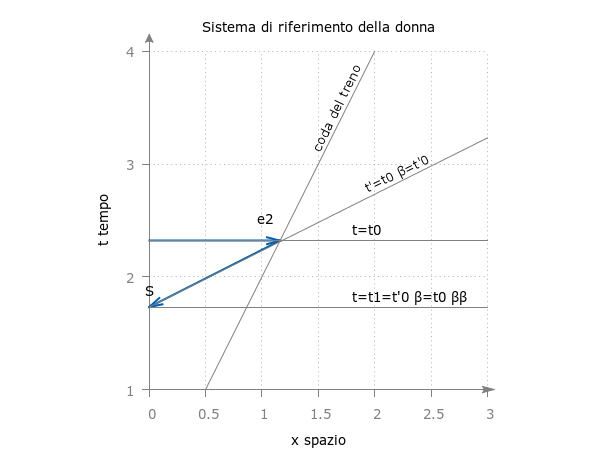
\includegraphics[scale=0.7]{figure/fig12}
 \caption{relatività galileiana}
\end{figure}

Ripercorriamo il ragionamento dal punto di vista  della signora per l'evento $e2$ tenendo d'occhio il grafico qui sopra. Vi ricordate? È il momento in cui la luce torna al passeggero.

\begin{enumerate}
 \item In $e2$ l'orologio della signora segna un certo tempo $t_0=2.32$ secondi, come sappiamo
 \item In quel momento $t_0$ il passeggero si trova in $e2$
 \item Il suo orologio in quel momento segna il tempo $t'_0 =t_0\beta=2$ che è minore di $t_0$.
\end{enumerate}

Vediamo adesso invece come stanno le cose per il passeggero:

\begin{enumerate}
 \item In $e2$ l'orologio del passeggero segna $t'_0=2$ 
 \item In $t'_0$ la signora si trova in $S$, con $x=0$ o $x'=-vt'_0$, sulla pensilina insomma
 \item In quel momento l'orologio della donna segna il tempo $t_1 =t'_1\beta$ che è minore di $t'_0$.
\end{enumerate}

Quindi bisogna sempre confrontare tra loro gli orologi che si sono sincronizzati, a parole la storiella è questa: in $e1$ la signora ed il passeggero, nello stesso punto dello spazio, sincronizzano gli orologi. Quando si verifica l'evento $e2$, ovvero la luce torna al passeggero, se la donna potesse vedere l'orologio al polso del passeggero leggerebbe un tempo minore rispetto al suo. Se quando si verifica l'evento $e2$ il passeggero potesse vedere l'orologio al polso della donna vedrebbe un orario inferiore al suo.\footnote{Da notare come questi tempi si ottengano moltiplando il precedente per $\beta$. Infatti $t_0 \beta= t'_0$ e $t'_0 \beta= t'_1 = t_0 \beta^2$. }


\section{Relatività del tempo, 4}

TODO Futuro per te, presente per me.
La simultaneità è solo dedotta, non toccata con mano.
Il figlio prima della madre? Causalità e cono di luce


\section{Misurare le lunghezze, 2}

A questo punto dovremmo essere piuttosto persuasi che il tempo possa anche essere relativo senza che il mondo sprofondi nel caos e nell'incoerenza: se ci muovessimo ordinariamente a velocità elevatissime la cosa sarebbe emersa da sempre e sarebbe forse palese per tutti.

Parlando di misura di lunghezza, qualche paragrafo più indietro, eravamo d'accordo che per una corretta misurazione gli estremi dell'oggetto devono essere considerati contemporaneamente. Nel dubbio tornate indietro a rinfrescarvi il concetto.

Però, va da sé, che se due osservatori possano non concordare sulla simultaneità, be' allora necessariamente si troveranno a non concordare sulle lunghezze.

Verifichiamo la lunghezza del treno per la donna sulla pensilina: nello stesso istante $t=0$ in cui la coda del treno la incrocia la locomotiva sarebbe $c \beta$, quindi il treno per la donna è più corto: lo spazio è relativo!

Anche in questo caso come per la velocità ed il tempo, non stiamo parlando di uno scherzo dei numeri, di un problema teorico: per entrambi gli osservatori ogni lunghezza nella direzione del movimento sarebbe più corta di quella misurata dall'altro. Se la nostra donna potesse vedere nel treno in movimento non solo vedrebbe tutto muoversi all'interno lentamente (dilatazione del tempo) ma vedrebbe anche ogni misura nella direzione del moto più corta (contrazione dello spazio), con il naso del passeggero più corto e la distanza tra la nuca ed il naso più breve. La distanza tra le spalle sarebbe invece uguale perché non si trova nella direzione del moto.

Ovviamente anche per il passeggero la donna e tutta la pensiline sarebbero più corte nella direzione del moto. Anche in questo caso non si tratta di un trucco: il treno è davvero più corto e potrebbe stare chiuso in un hangar più corto di $c$ (purché continui a muoversi, però!). 

Vediamo graficamente come passare da una misura ad un altra.

TODO Relatività delle dimensioni
%\begin{figure}[h!]
% \centering
% \includegraphics[scale=.09]{materiale/rel-distanze}
% \caption{Relatività lunghezze}
%\end{figure}


\section{Relatività Speciale}

A questo punto dovremmo avere assimilato cosa significa relatività di spazio e tempo così come intendere lo spazio-tempo: possiamo riportare tutti i dati dell'esperimento della luce con cui abbiamo introdotto il capitolo per poterlo confrontare con l'esperimento della pallina.

\begin{center}
\begin{tabular}{>{\itshape}l >{\itshape}c >{\itshape}c }
\toprule
            & \textbf{donna} & \textbf{passeggero} \\
velocità treno            & $v$        & $0$  \\ 
velocità pensilina        & $0$        & $-v$  \\
velocità pallina          & $c$        & $c$  \\
secondi dell'esperimento  & $2.32$     & $2$  \\
percorso pallina          & $2c \beta$       & $2c$  \\
lunghezza del treno       & $c\beta$   & $c$  \\
\bottomrule
\end{tabular} 
\end{center}

Sono i risultati sperimentali che portano a concepire la relatività dello spazio e del tempo. Infatti se la velocità della luce è la medesima, essendo la velocità pari allo spazio diviso il tempo, necessariamente tempi e distanze devono modificarsi proporzionalmente. Rimane invariante invece lo spazio-tempo.


\section{Conclusioni}

In queste pagine abbiamo provato a fornire una presentazione gentile ma rigorosa da un punto di vista matematico della teoria della relatività speciale di Einstein. Siamo riusciti utilizzando solo le quattro operazioni a spiegare gli effetti di dilatazione del tempo e contrazione dello spazio, ricorrendo ad un esperimento e diversi esempi. Abbiamo poi mostrato quali fossero i calcoli sottesi mostrando, in appendice, tutti i passaggi e ricorrendo a quel po' di algebra imparata in terza media.

Da qui in poi il lettore interessato potrà completare quanto appreso rinunciando alle unità di misura relativistiche e poi affrontando il non facile modello della teoria della relatività generale in cui si studiano gli effetti gravitazionali sul moto dei corpi. 
